\chapter{\MakeUppercase{Управление по положению схвата. Аналитический метод. }}

Расчет углов в сочленениях производится с помощью результатов точного аналитического решения обратной задачи о положениях:
\begin{align*}
    X_{1A}&=d_1+l_2\sin\varphi_2+l_3\sin{(\varphi_2+\varphi_3)} \\
   Z_{1A}&=l_1+l_2\cos\varphi_2+l_3\cos{(\varphi_2+\varphi_3)} \label{eq:graph} \tag{1}
\end{align*}

\begin{figure}[ht!]
    \centering
    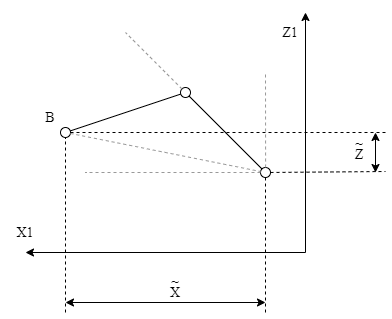
\includegraphics[width=0.5\textwidth]{chapter_x1/figure1.png}
\end{figure}

Преобразуя данные уравнения, получим:
\begin{align*}
    l_2\sin\varphi_2+l_3\sin{(\varphi_2+\varphi_3)}&=X_{1A}-d_1=\tilde X \\
   l_2\cos\varphi_2+l_3\cos{(\varphi_2+\varphi_3)}&=Z_{1A}-l_1=\tilde Z \\
   \tilde l=\sqrt{\tilde X^2+\tilde Z^2} \\
   \alpha=\pi-\varphi_3
\end{align*}
По теореме косинусов:
\begin{align*}
    \tilde l^2 &= l_3^2+l_2^2-2 l_2 l_3 \cos\alpha\\ 
     \cos\varphi_3 &= \frac{\tilde l^2-l_3^2-l_2^2}{2l_2l_3}=\frac{(\tilde X^2+\tilde Z^2)-(l_3^2+l_2^2)}{2l_2l_3}=D
\end{align*}
Замечание: если $|D|>1$, то программное движение нереализуемо, так как координаты целевой точки вне рабочей области.
$$\varphi_3=\pm \arccos{D+2\pi n}, n\in\zeta$$

%?? дополнительный рисунок ?? 
Найдем $\varphi_2$:
\begin{align*}
\tg\beta&=\frac{\tilde Z}{\tilde X} \\
\beta&=\arctan{(\tilde Z,\tilde X)}
\end{align*}

По теореме косинусов:
\begin{align*}
    l_3^2 &= \tilde l^2+l_2^2-2\tilde l l_3 \cos\gamma \\
    \cos\gamma &= \frac{\tilde l^2+l_2^2-l_3^2}{2\tilde l l_2} \\
    \gamma &=\pm \arccos\frac{\tilde l^2+l_2^2-l_3^2}{2\tilde l l_2}
\end{align*}
$$\varphi_2+\gamma+\beta=\frac\pi 2$$ 

Тогда $$\varphi_2=\frac \pi 2 -\gamma-\beta.$$

Для проверки результата решим прямую задачу. Полученные значения $\varphi_2,\varphi_3$ подставим в \eqref{eq:graph}. 

Программа для нахождения $\varphi_2,\varphi_3$, а также графики реальных и программных значений координат представлены в Приложении 1.

Также были получены квадратичные отклонения: 
$$||X(t)-X^*||_2=4.98\cdot10^{-16}$$
$$||Z(t)-Z^*||_2=4.65\cdot10^{-16}$$.